\chapter{Fundamentals}
\label{chp:basics}
This chapter firstly describes the cooperative game and specifically explains all required mathematical definitions. It then presents six different game-theoretical solution approaches and how they are applied to solve the game.

\section{Game definition}
Firstly, the generic game definition is given. Additional definitions for each of the solution approaches are defined in the corresponding subsections of each solution.

According to \citet{holler2006einfuhrung} a game $G = (N,S,u)$ is defined by:
\begin{itemize}
\item
set of players $N = \{1,2\}$, in this case two players, where player 1 is the Engine and player 2 is the Motor.
\item
strategy space $S$, which is the set of all possible strategy combinations $s=(s_1,s_2)$ for each player, where $s\in S$. The strategy space contains two sets with all strategy combinations of that player.
\item
utility function $u = (u_1,u_2)$, where $u_i(s)$ for $i=1,2$ gives the utility (or also called payoff) for that player when the strategy combination $s$ is played.
\item
utility space (payoff space) which is the set of all possible utility combinations:
$P = \{u(s)|s \in S\} = \{(u_1(s),u_2(s),  \forall s \in S\}$
\end{itemize} 

Let us denote the number of pure strategies of each player with $n$ and $m$. Therefore, these constitute a bimatrix game, meaning that the payoffs of the game can be represented in two matrices of size $m \times n$. Let the payoff matrices $A$ and $B$ denote the payoffs for the first player, the engine, and the second player, the motor respectively, where $A = (a_{ij}: i \in \{1,...,n\}, j \in \{ 1,...,m\})$ and $B = (b_{ij}: i \in \{1,...,n\}, j \in \{ 1,...,m\})$. Sometimes player 1 is called the row player and player 2 is called the column player, since their strategies vary along the rows or along the columns of the matrices. The game is a non-zero sum game, since the sum of the two payoff matrices is not 0, $A + B \neq 0$.

As opposed to a non-cooperative game, in cooperative games the players are allowed to make binding agreements among themselves in order to achieve a better payoff, that is, they can form coalitions. We distinguish between the grand coalition of all players $N$ or $\{1,2\}$, where they all cooperate, and the individual coalitions $\{i\}, \forall i \in N$ which are $\{1\}$ and $\{2\}$. There is also the empty coalition, where neither cooperates, but this coalition is irrelevant to our purposes. Each coalition has a value associated with it. The grand coalition forms its value as a sum of the payoffs of the engine and motor multiplied element-wise by a matrix with weights. The weights are distributed according to the torque deviation which the engine and motor produce. The torque deviation is defined as the difference between the required and the actual torque at the current time step. When the deviation is 0, the payoffs are weighted by 0.99, when it is between 0-10\% of the required torque it is weighted by 0.991, when between 10-20\% weight is 0.992 and so on up to 1.0 (the full sum of engine and motor torque).


The goal of the game is to save fuel and to maintain low gas emissions while achieving the required torque at any moment in time. Therefore, the payoffs are penalties as opposed to benefits and they have to be minimized. All of the solutions have been defined by taking into account that this is a minimization problem. Most of the solutions applied in the literature work with maximizing payoffs, but for the purpose of this thesis their definitions and implementations have been modified to minimize the two payoff functions instead. 


There exist two types of cooperative games - with transferable and with non-transferable utility. In transferable utility (TU) games the payoff of one player can be transferred to another player without any loss. In contrast, in non-transferable utility (NTU) games the payoffs of each player cannot be redistributed among the other players. In this thesis the payoffs of the engine and the motor are not interchangeable, since decreasing the payoff of one player does not mean increasing the payoff of the other player at the same time. Therefore, their payoff functions are thought to be independent from each other.

The payoff functions are constructed in the following way. The engine payoff is:
\begin{equation}
\begin{split}
a_{ij} = w_1 \times fuelConsumptionRate + w_2 \times | requiredTorque - actualTorque | + \\
w_3 \times HCemissions + w_4 \times COemissions + w_5 \times NOXemissions + \\
w_6 \times fuelConsumed
\end{split}
\end{equation}
Where the fuel consumption rate is in grams per second (\textit{gps}), the difference between required and actual torque is in Newton meters (\textit{Nm}), the gas emissions are all in \textit{gps} and the consumed fuel from the beginning of the simulation up to this time step is in liters. The motor payoff is:
\begin{equation}
\begin{split}
b_{ij} = w_2 \times | requiredTorque - actualTorque | + w_7 \times powerConsumed\\
w_8 \times SOCdeviation
\end{split}
\end{equation}
Where the consumed power is in \textit{kW} from the beginning of the simulation and SOC deviation is the difference between the target SOC of 70\% and the current SOC of the battery.

To summarize, the game defined is a two-player cooperative bimatrix non-zero-sum game with non-transferable utility.

\section{Game-theoretical solution approaches}
This thesis examines a variety of solution approaches for cooperative games which are later applied and simulated as described. These include Pareto Optimality, Nash Equilibrium, Nash bargaining solution, Kalai-Smorodinsky bargaining solution, the Core and the Shapley value.

\subsection{Pareto Efficiency and Pareto Optimality}
In the literature two terms are often used to refer to the same concept - Pareto Efficiency and Pareto Optimality. However, they are used with distinct meanings throughout this thesis. Pareto Efficiency denotes an allocation of resources such that no player can improve their outcome without impairing another player. In the strategy space of the game there can exist more than one Pareto efficient outcome. Therefore, we define a Pareto optimal outcome, or Pareto Optimality, as the single best outcome from the set of all Pareto efficient outcomes. The criteria for determining the best outcome is as follows. All Pareto efficient points are compared by their torque deviation and the point with the least torque deviation is taken as the Pareto optimal point. Torque deviation is defined as the absolute difference between the required and the actual torque at this stage of the game. If more than one outcomes have the same torque deviation the outcome with the smallest fuel consumption rate is taken as a second criterion. Similarly, if more than one outcome have the same fuel consumption rate the one with the smallest power consumed by the motor is taken. This is the third and last criterion.

\subsection{Nash Bargaining solution}
The Nash Bargaining solution or shortly the Nash solution was defined by \citet{nash1950bargaining}. It considers the game as a bargaining game where each player requests some portion of the existing good, in this case torque. A bargaining game $G$ is defined by specifying a conflict point $c = (c_1,c_2)$ in addition to the payoff space $P$, comprising of the two payoff vectors as defined above $u = (u_1,u_2)$. The pair is denoted as $(P,c)$ as in \citet{holler2006einfuhrung}. The conflict point is the point where both players do not cooperate with each other. There exists a common misinterpretation because the word "conflict" point itself implies a point where both players face a disagreement and hence their payoffs are the worst. A Nash Equilibrium does not present such a worst case and therefore the term conflict point may seem misleading, but for the sake of consistency in the literature, the term will be kept as it is. Since the conflict point in the literature is often taken to be the Nash Equilibrium of the corresponding non-cooperative game, the next subsection deals with an algorithm to find a Nash Equilibrium.

Taking these into account, a Nash Bargaining solution is the vector $u^*$ from the set $P$:
\begin{equation}
NP^* = max(c_1 - u_1^* )(c_2 - u_2^*)
\end{equation}

so that $u^* = (u_1^*,u_2^*) \in P$ and $u_i^* < c_i$ for $i = 1,2$, meaning that the Nash solution point $u^*$ payoff is less than the conflict point payoff. The main idea of the Nash solution expressed graphically as in \ref{fig:nashSol} is to maximize the product of the differences between the conflict point and the Nash solution point coordinates in 2D.

\begin{figure}[h]
\centering
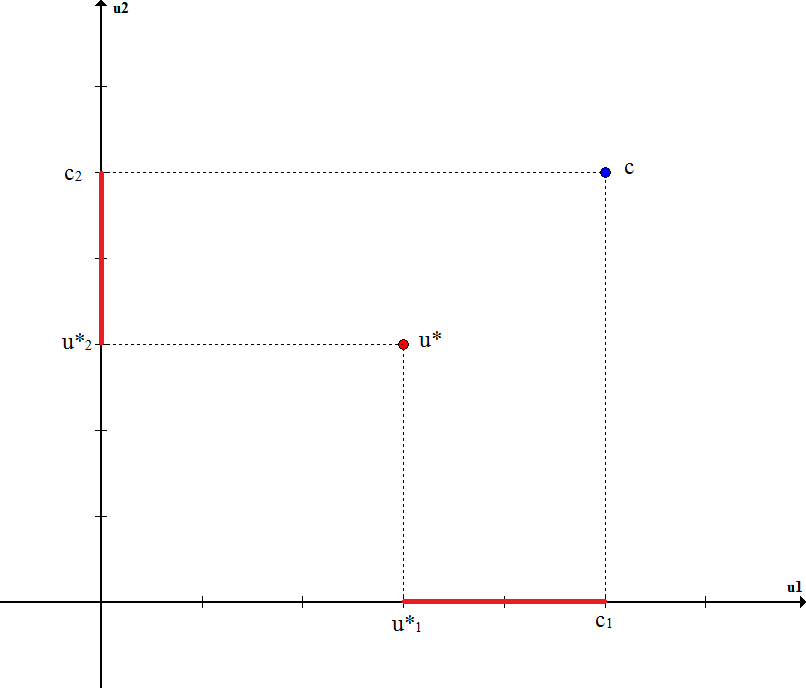
\includegraphics[scale=0.5]{figures/nashSolution}
\caption{Maximized Nash Product}
\label{fig:nashSol}
\end{figure}

The Nash solution is characterized by four axioms as defined in \citet{holler2006einfuhrung}. 

The first axiom is called Invariance with Respect to Affine Transformations of Utility. Given a bargaining game $(P,c)$ and two random real numbers $a_i > 0$ and $b_i$, where $i = 1,2$ for both players, it is true that $f_i(P',c') = a_i f_i(P,c) + b_i$. This holds if $(P',c')$ is a game resulting from a linear transformation which preserves the order of all points $u$ and $c$ from $P$ so that $y_i = a_i x_i + b_i$ and $c_i' = a_i c_i + b_i$, where $y \in P'$ and $c' \in P$. In other words such a linear transformation of the game space does not affect the solution of the bargaining game.

The second axiom is Symmetry. If $(P,c)$ is a symmetric bargaining game then $f_1(P,c) = f_2(P,c)$. A game is symmetric if $c_1 = c_2$ and if $(u_1, u_2)$ and $(u_2, u_1)$ are both in the payoff space $P$. This results in a conflict point lying on the 45\textdegree  line from the origin of the coordinate system. $P$ is symmetric with regard to this line. This axiom tells that if the payoffs of the two players can be interchanged and the game does not change as a consequence of that, then its solution should also not distinguish between the two players.

The third axiom is Independence of Irrelevant Alternatives. It states that $f(P,c) = f(Q,c)$ if two games $(P,c)$ and $(Q,c)$ have the same conflict point $c$, $P \subseteq Q$ and $f(Q,c) \in P$. Therefore, only the conflict point is relevant, because if the payoff space of the game is extended to a superset or it is shrunk to a subset, then the solution itself does not change.

The last axiom is the Pareto Optimality. For a bargaining game $(P,c)$ there is no $x \neq f(P,c) \in P$ such that $x_1 \leq f_1(P,c)$ and $x_2 \leq f_2(P,c)$, which is an example of group rationality.

\subsection{Nash Equilibrium and Lemke-Howson algorithm}
One of the most popular algorithms for finding a Nash Equilibrium for bimatrix non-zero-sum games is the Lemke-Howson algorithm \citep{lemke1964equilibrium}. The Matlab implementation developed by \citet{lemkeHowson2014Matlab} was utilized to find one Nash Equilibrium in mixed strategies. This function contains a parameter, which affects the final result of the algorithm. Changing the parameter yields different Nash equilibria as output. This parameter $k$ is the initial pivot, a number between 1 and $n+m$, where $n$ and $m$ are the number of strategies of player 1 and player 2 respectively. The general idea of the the algorithm is that it works on two graphs containing nodes and edges, one graph per player. It starts at the (0,0) point. It selects a $k$, the pivot, or the label of the graph, containing the strategy to be dropped first when traversing the graph. From there a path to the end is followed in order to find a Nash Equilibrium. 

There a number of reasons for the different Nash Equilibrium solutions that the algorithm produces. According to \citet{lemke1964equilibrium} there exist an odd number of Nash Equilibria in any nondegenerate game. A nondegenrate game is a game where no mixed strategy with a support of size $k$ has more than $k$ pure strategies \citep{nisan2007algorithmic}. Moreover, a support of a mixed strategy is defined as the set of pure strategies with positive probabilities. Since there is an odd number of Nash Equilibria, there must be at least one Equilibrium, which proves that the algorithm will always find one solution in mixed strategies. However, which of all Nash Equilibria is found depends on which strategy label is dropped first. The initial pivot label which the algorithm drops can belong to either of the two players and be any of their $n$ or $m$ strategies.

As discussed in \citet{shapley1974note} the Lemke-Howson algorithm possesses a significant weakness, namely that it is neither guaranteed that the algorithm will find all possible solutions, nor that it will tell if there are any unfound solutions.

The fundamentals of the Lemke-Howson algorithm are described next. Let us assume a scenario of a 2-player bimatrix game as the one used throughout this thesis, where the players $1$ and $2$ each have $n$ and $m$ number of pure strategies and their payoffs are in the matrices $A = (a_{ij}: i \in \{1,...,n\}, j \in \{ n+1,...,n+m\})$ and $B = (b_{ij}: i \in \{1,...,n\}, j \in \{n+1,...,n+m\})$ respectively. The mixed strategies are the vectors $s=(s_1,s_2...,s_n)$ and $t=(t_{n+1},t_{n+2},...,t_{n+m})$ where $S = \{s \geq 0; \sum_{i=1}^{n}s_i = 1\}$ and $T = \{t \geq 0; \sum_{j=n+1}^{n+m}t_i = 1\}$ are the sets for the mixed strategies spaces. Then, the payoff for player 1 is $\sum_{i=1}^{n}\sum_{j=n+1}^{n+m} a_{ij} s_i t_j$ and the payoff for player 2 is $\sum_{i=1}^{n} \sum_{j=n+1}^{n+m} b_{ij} s_i t_j$. An equilibrium is a pair of strategies $(s^*,t^*)$ satisfying:
\begin{equation}
\sum_{i=1}^{n} \sum_{j=n+1}^{n+m} a_{ij}s_i^*t_j^* = \max_{s \in S} \sum_{i=1}^{n} \sum_{j=n+1}^{n+m} a_{ij}s_i t_j^*
\end{equation}
\begin{equation}
\sum_{i=1}^{n} \sum_{j=n+1}^{n+m} b_{ij}s_i^*t_j^* = \max_{t \in T} \sum_{i=1}^{n} \sum_{j=n+1}^{n+m} b_{ij}s_i^* t_j
\end{equation}


If we also define the sets:
\begin{equation}
\tilde{S} =  S \cup \{ s \geq 0: \sum_{i=1}^{n} s_i \leq 1 \text{ and } \prod_{i=1}^{n} s_i = 0 \}
\end{equation}

\begin{equation}
\tilde{T} = T \cup \{t \geq 0: \sum_{j=n}^{n+m} t_i \leq 1 \text{ and } \prod_{j=n}^{n+m} t_i = 0 \}
\end{equation}
this allows us to define closed convex polyhedral regions $S^i$ and $S^j$ which together form $S^k \in \tilde{S}$:
\begin{equation}
S^i = \{ s \in \tilde{S}: s_i = 0 \} \text{ for } i \in \{1,...,n\}
\end{equation}


\begin{equation}
S^j = \{ s \in S: \sum_{i=1}^{n} b_{ij} s_i = \max_{l \in \{n+1,...,n+m\}} \sum_{i=1}^{n} b_{il} s_i \} \text{ for } j \in \{n+1,n+2,...,m\}
\end{equation}


$S^i$ contains all $\tilde{S}-S$ and $S^j$ contains the mixed strategies for player 1 and the pure strategy $j$ of player 2 which is his best outcome. $S^i$ and $S^j$ both make $S^k$ and cover the whole set $\tilde{S}$. The same can be applied to define the regions $T^k \in \tilde{T}$:
\begin{equation} 
T^i = \{ t \in T: \sum_{j=n+1}^{n+m} a_{ij} t_j = \max_{l \in \{1,...,n\}} \sum_{j=n+1}^{n+m} a_{lj} t_j \} \text{ for } i \in \{1,...,n\} 
\end{equation}

\begin{equation}
T^j = \{ t \in \tilde{T}: t_j = 0 \} \text{ for } j \in \{n+1,...,n+m\} 
\end{equation}


The Lemke-Howson algorithm represents the strategies of both players in two graphs with nodes and edges. The already mentioned definitions are required in order to define a labelling for the graphs. A labelling of a node consists of all of the labels of all surrounding regions of this node. Let the nonempty label of $s \in \tilde{S}$ be $L'(s) = \{ k: s \in S^k \}$ and similarly the nonempty label of $t \in \tilde{T}$ be $L''(t) = \{ k: t \in T^k \}$ and the label of the node pair with pure strategies $(s,t) \in \tilde{S} \times \tilde{T}$ be $L(s,t) = L'(s) \cup L''(t)$. A node pair $(s,t)$ is completely labelled whenever $L(s,t) = K$, meaning that it contains the labels for all regions $k \in K$. A node pair is almost completely labelled if $L(s,t) = K - \{k\}$ for some $k \in K$. 

Then, as in \citet{shapley1974note} a node pair $(s,t) \in S \times T$ is an equilibrium point of (A,B) if and only if $(s,t)$ is completely labelled. Let the two graphs be $G' \in \tilde{S}$ and $G'' \in \tilde{T}$. Two nodes are adjacent if they are on the two ends of the same edge which means that their labels differ in exactly one element. The set of k almost completely labelled nodes in the graphs and their edges are the disjoint paths of the graph and cycles. The equilibria of the game are always located at the end of these paths. Also, the starting node, by default (0,0) is called an artificial equilibria and it is also located at the end of a path.

The algorithm works by starting at $(s,t) = (0,0) \in G' \times G'' $. Then a label $k$, which is to be dropped from $(s,t)$, is chosen (initial pivot). This $k$ can belong to either $n$ or $m$. Let this node be $(s,t)$ and its new label (after dropping $k$) be $l$. Then, if $l=k$ a Nash Equilibrium is reached. If $l\neq k$, then the algorithm continues by dropping another label and continuing until a completely labelled node has been reached, which is an equilibrium point. The starting label to drop is the pivot parameter as in the Matlab implementation. Since there are $n+m$ labels (strategies) which can be dropped first and they can end up in a different Nash Equilibrium node in the graph, it is inefficient to experiment with all different starting strategies. Experiments were done with $1$, $\frac{n+m}{4}$, $\frac{n+m}{2}$, $\frac{3(n+m)}{4}$ and $n+m$ as the first strategy to be dropped. In order to choose which point to use, the Matlab implementation NPG from \citet{npg} was used the Lemke-Howson solution with the $k$ strategy, which was closest to the NPG solution was chosen. This $k$ was $\frac{n+m}{2}$, which was passed to the Lemke-Howson algorithm as an input.

\subsection{Kalai-Smorodinsky Bargaining Solution}
The Nash Bargaining solution has the significant disadvantage that it is not monotonic. The third of the four axioms defined above Independence of Irrelevant Alternatives was criticized as in \citet{kalai1975other}. Therefore, \citet{kalai1975other} propose another unique bargaining solution called the Kalai-Smorodinsky solution. They replace the third axiom with another axiom for Individual Monotonicity, which the Nash solution does not conform to. 

The axiom states that if for two bargaining games $(P,c)$ and $(R,c)$ such that $P \subset R$ the equation $m_i(P) = m_i(R)$ holds for player $i$, then for player $j \neq i$ it is true that $f_j(R,c) \geq f_j(P,c)$.

$m_i(P,c)$ and $m_i(R,c)$ denote the minimum payoffs for players $i = 1,2$. They are defined as $m_i(P) = min(u_i | (u_1,u_2) \in P$. The point $m(P) = (m_1(P),m_2(P))$ is called the ideal point of the game, because that is where both players achieve minimum payoffs; hence, the ideal outcome of the game. However, often this point is not feasible. As in the Nash solution, the conflict point is also crucial in the Kalai-Smorodinsky solution. A further term is required and this is the Utility Boundary of the utility space $P$ of a game:


Consequently, the Kalai-Smorodinsky solution is defined as follows:
\begin{equation}
\frac{c_2 - u_2}{c_1 - u_1} = \frac{c_2 - m_2}{c_1 - m_1}
\end{equation}

so that
\begin{equation}
u_i \leq v_i, \frac{c_2 - v_2}{c_1 - v_1} = \frac{c_2 - m_2}{c_1 - m_1} 
\end{equation}

where $(v_1,v_2) \in P$. The pair $(u_1,u_2)$ is the Kalai-Smorodinsky solution. As \citet{kalai1975other} point out, this solution is graphically represented as the intersection point of the line $L(c,m)$ and the utility (payoff) boundary $H(P)$ as shown in Figure \ref{fig:ksSol}. $L(c,m)$ is the line connecting the conflict point $c$ and the ideal point $m$. The utility boundary $H(P)$ or also called the Pareto frontier is defined as the set of all Pareto efficient points. For all random payoffs of one player the boundary gives the minimal possible payoff of the other player. If the Pareto frontier only contains one Pareto efficient point then the Kalai-Smorodinsky solution is the ideal point itself $u* = m(P)$.

\begin{figure}[h]
\centering
\includegraphics[scale=0.5]{figures/kalaiSmorodinskySolution}
\caption{Kalai-Smorodinsky Solution}
\label{fig:ksSol}
\end{figure}

\subsection{Core}
As opposed to the previous four solution approaches, which treated the game as individually cooperative, the next two approaches the Core and the Shapley value regard the game as a coalitional game. The difference is that the previous approaches were applicable to 2-player individually cooperative games only, whereas the Core and the Shapley value can additionally be extended to coalitional n-player games. However, this thesis only deals with 2-player games and therefore does not need this extension. Moreover, there is a crucial distinction between the Core and the Shapley value because the Core produces a set of points as a solution, while the Shapley value is always only one single point. For this reason the Core is similar to the Pareto efficiency concept because both can contain more than one point. A single point from this set needs to be chosen and the criteria for choosing a single solution from the Core is the same as in the case of Pareto efficiency - torque deviation, fuel consumption rate and power consumed by the motor are taken into account.

To define the core of a game, a new term called imputation is introduced. An imputation is such an allocation of resources that is both individually rational and group rational (or Pareto efficient). For transferable utility (TU) games individual rationality means that each player in the coalition receives at most the payoff that they would receive on their own expressed as $u_i \leq v(\{i\})$. Group rationality, which is equivalent to efficiency and in our case also to Pareto efficiency, means that the sum of the payoffs of all players in the grand coalition is the value of the game, $\sum_{i=1}^{N} u_i = v(N)$. For non-transferable utility (NTU) games such as ours a payoff vector $u$ is an imputation when there is no vector $u'$ which strictly dominates it. This is expressed by $u' \in V(N)$ such that $u'_i < u_i, \forall i\in N$. According to \citet{holler2006einfuhrung} a vector $u'$ is said to dominate another vector $u$ with regard to the coalition $K$ if $u'_i \leq u_i, \forall i \in K$ and for at least one $i \in K$ the inequality $u'_i < u_i$ holds when $u' \in V(K), u \in V(K)$.

After describing the notion of imputation, the core $C$ of a game $G$ is the defined as the set of all non-dominated imputations:
\begin{equation}
C(G) = \{u \;|\; v(K) - \sum u_i \leq 0, \; \forall i \in K, \; \forall K \in N \}
\end{equation}

If an imputation $x$ is in the core $x \in C(G)$ then for all coalitions $K \in N$ there is no other coalition $K$ for which another imputation $y$ dominates $x$ denoted as \textit{y dom x via K} \citep{holler2006einfuhrung}. Therefore, no coalition can make its participants better by substituting $x$ with $y$; hence, $x$ is thought to be coalitionally rational. There are two different possibilities when this can be true. There is either no coalition at all which can realize $y$, or $y$ is worse than $x$ meaning that it is not true that $y_i < x_i$ for at least one $i \in K$ and $y_i \leq x_i$ for all $i \in K$. 

Since all imputations in the core are not dominated by any other imputation, the core is internally stable. The core of a game can be empty or can contain many imputations. This comes from the fact that the relation \textit{dom} is not transitive; hence, if it is true that an imputation $x$ dominates $y$ and $y$ dominates $z$, this does not imply that $x$ dominates $z$.

\subsection{Shapley Value}

The Shapley value of a game with transferable utility according to \citet{holler2006einfuhrung} is defined as:
\begin{equation}
\label{eq:shapley}
\Phi_i(v) = \sum_{i \in K, K \subset N} \frac{(k-1)!(n-k)!}{n!} [ v(K) - v(K - \{i\})],
\end{equation}

\begin{equation}
\sum \Phi_i(v) = v(N), \; \Phi(v) = (\Phi_i(v))
\end{equation}
$k$ denotes the number of players in coalition $K$ and $n$ is the total number of players. $v(K)$ is the value of the coalition $K$, whereas $v(K - \{i\})$ is the value of the coalition $K$ without the player $i$. The sum of the Shapley values of all players must equal the total value of the game, which is also the value of the grand coalition.

The Shapley value was introduced by \citet{shapley1952value} where it is described that the game must be represented by its characteristic function $v: 2^N	\rightarrow \mathbb{R}$. In addition, the Shapley value is the single point which satisfies the following three axioms.

The first axiom is Group Rationality or Efficiency, which is equivalent to Pareto efficiency. This axiom was already described in the subsection of Nash bargaining solution. The second axiom is Symmetry and it states that if the players change their order then the values of the players change accordingly. Therefore, the number of players does not have an influence on the value which that player receives. The third axiom is based on the assumption $\Phi_i(v+w) = \Phi_i(v) + \Phi_i(w)$ where $v+w$ is the combination of two games $v$ and $w$.

In general the Shapley value is about permutations of the players and especially who arrives first or who is able to make the decision first. The order of the players is irrelevant and each different order has the same probability. The equation \ref{eq:shapley} is.
On the one hand, a player who has an influence on the value of the coalition, is called a crucial or pivot player. For such a player $i$ this is true whenever $K$ is a winning coalition and $K-\{i\}$ is a losing coalition. On the other hand, a player is called a dummy player when a coalition $K$ has the same value regardless whether $i$ is in it or not - $[v(K) - v(K-\{i\})]$.